
%%% Local Variables:
%%% mode: latex
%%% TeX-master: "../Tesis"
%%% End:
\chapter{Particle Accelerators}
\label{c:accel} % For referencing the chapter elsewhere, use \ref{} 
\lhead{Chapter~\ref{c:accel}.
  Accelerators} % This is for the header on each page - perhaps a shortened title
Particle accelerators are machines whose name is self explanatory. They were
originally developed for nuclear physics. Although we could argue that a
cathodic tube is an accelerator itself, we count as the first accelerator one
that was designed, after Rutherford challenged the scientific community in 1927
to accelerate charged particles to energies higher than natural
$\alpha$-decays\cite{Steere2005timeline}, which have a typical energy of
\SI{5}{MeV}.
% Cockcroft-Walton
This accelerator was the Cockcroft-Walton multiplier, which was used to produce the first ever reported nuclear fission. The original setup
is shown in Fig.~\ref{fig:cock}. It consisted of an AC power source charging a
ladder of capacitors by means of diodes, generating a large voltage
output\cite{Cockcroft619}. Following the relation between the electric field
($\vec{E}$) and the scalar potential ($V$): $\vec{E}=-\nabla{V}$ and equating
Newton's second law of motion ($\vec{F}=m\vec{a}$) to the Lorentz force
($\vec{F}=q(\vec{E}+\vec{v}\times\vec{B})$) we infer that the acceleration in an
electrostatic accelerator such as the Cockcroft-Walton is:
$\vec{a}=-\frac{q}{m}\nabla{}V$. Ever since, accelerators have not stopped
evolving. Scientists kept building larger and larger accelerators until they hit
a limit with electrostatic fields due to voltage breakdown\cite{EASTHAM1984101}.
% I poupusefully missed the van der graff generator

\begin{figure}
\centering
 \begin{minipage}{\textwidth}
 \centering
  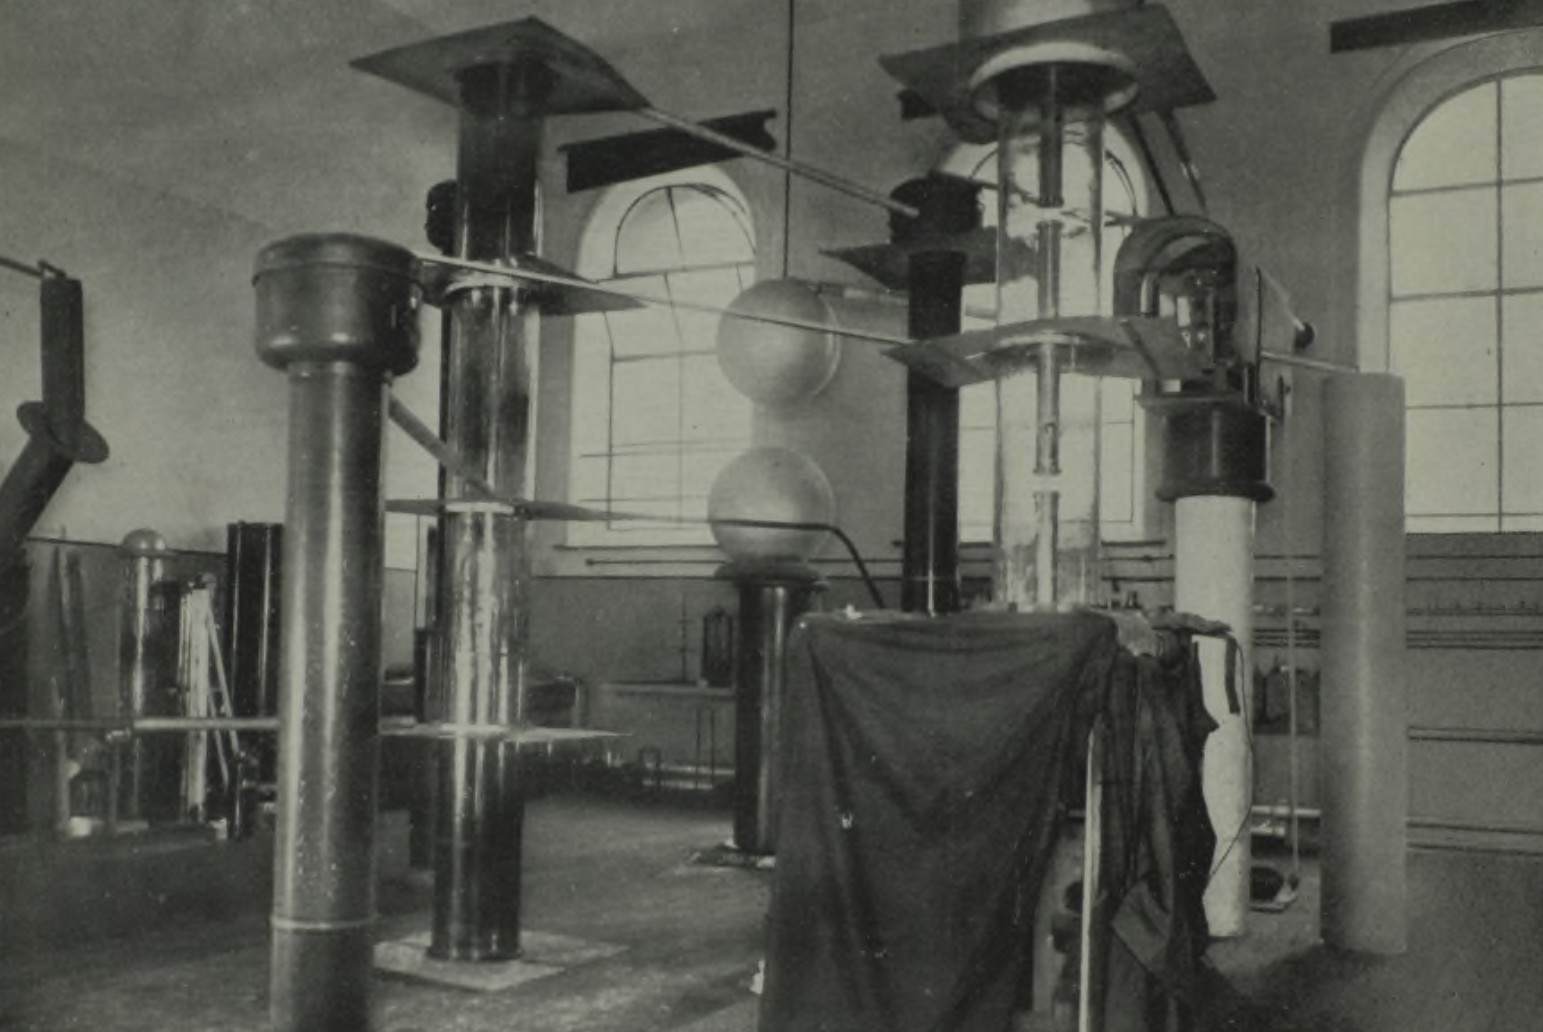
\includegraphics[width=3.5in]{Pictures/cockroft.jpg}
  \caption{\label{fig:cock}
   	Cockcroft-Walton accelerator original setting.}
   	\footnotesize{Picture taken from \citep{Cockcroft619}}
   \end{minipage}
\end{figure}
% RF Accelera6tors
% LINACS
A new technique for accelerating charges emerged. Already in 1924 Gustav Ising
had proposed using drift tubes to shield the charged particle from a pulsed
voltage\cite{Ising}, and in 1928 Rolf Wider\"oe suggested using a radiofrequency
(RF) system \cite{Wideroe1928}. To prove this principle Wider\"oe built the
first linear accelerator or linac, and RF acceleration was born.
%Cyclotron
Using the RF acceleration principle and one of Wider\"oe's ideas, Ernest
Lawrence set electrons in a curved path by applying a perpendicular magnetic
field so that the electrons would pass several times through and accelerating
gap. Figure \ref{fig:cyclo} shows Lawrence drawings in his 1934 patent and in
Fig. \ref{fig:lawrence} we see Lawrence standing next to his \SI{1.5}{m}
diameter cyclotron in the University of California at Berkeley.
\begin{figure}
 \centering
  \begin{minipage}{\textwidth}
  \centering
   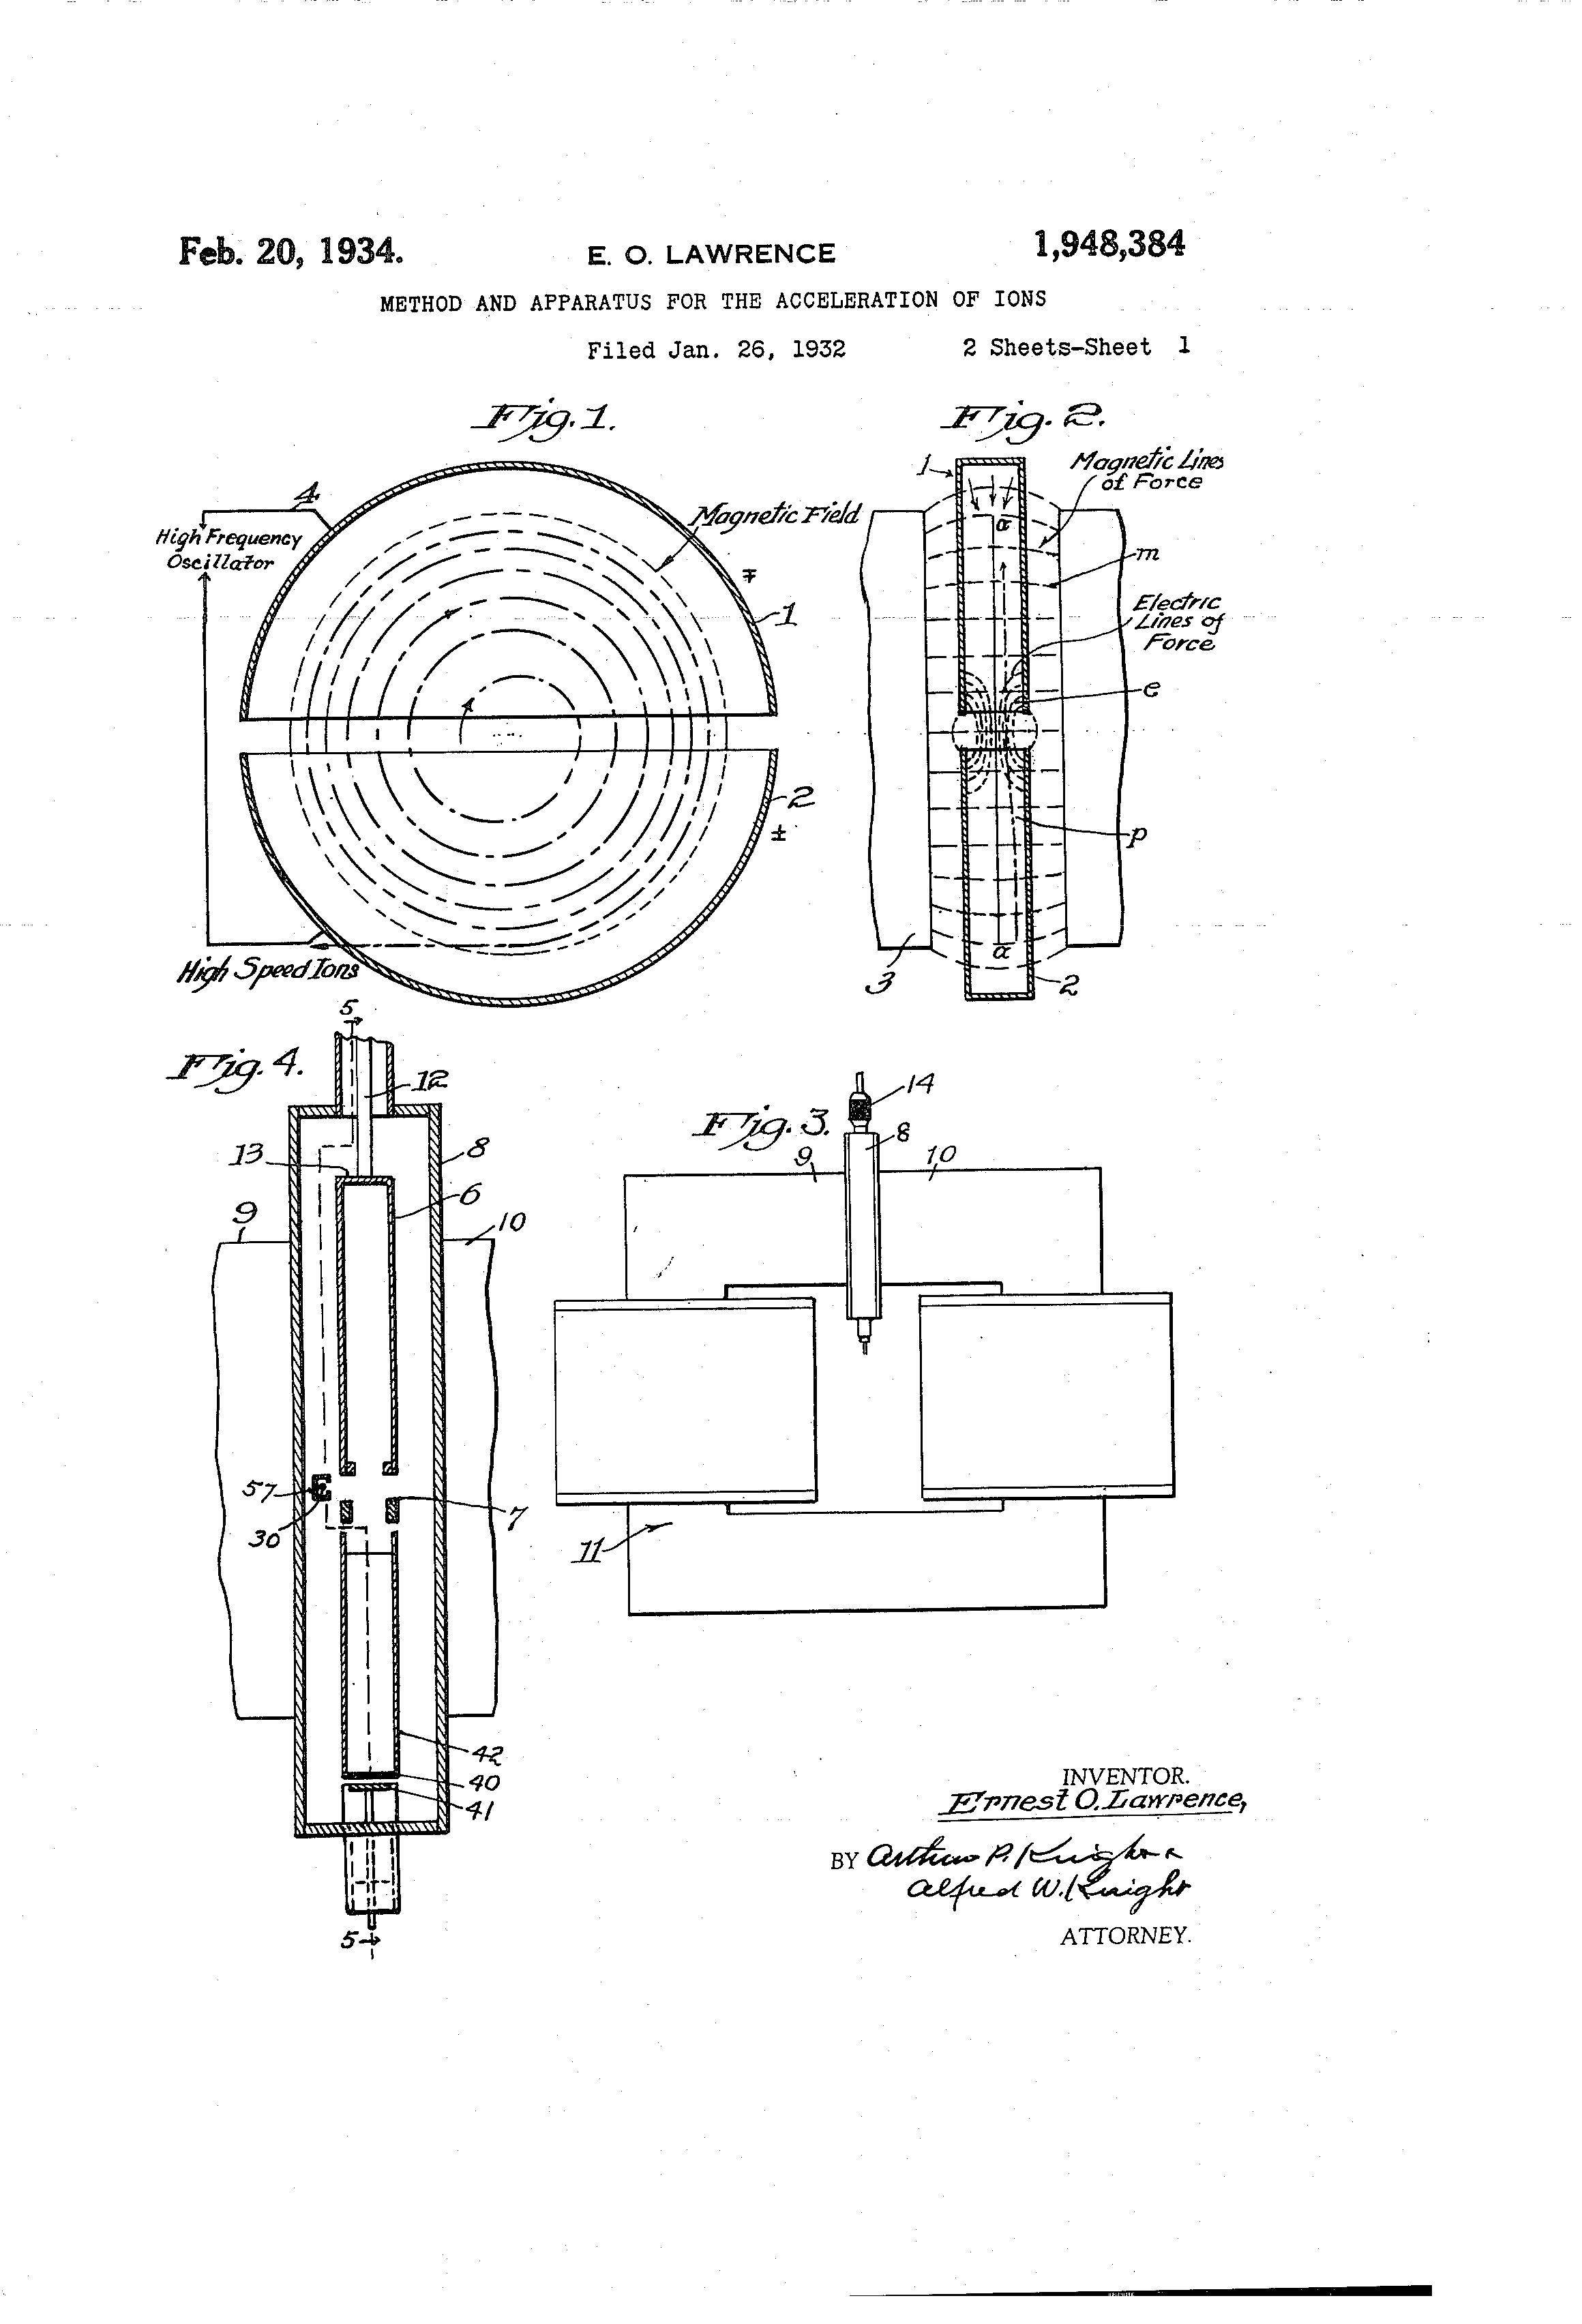
\includegraphics[width=.49\textwidth]{Pictures/cyclo1.png}
   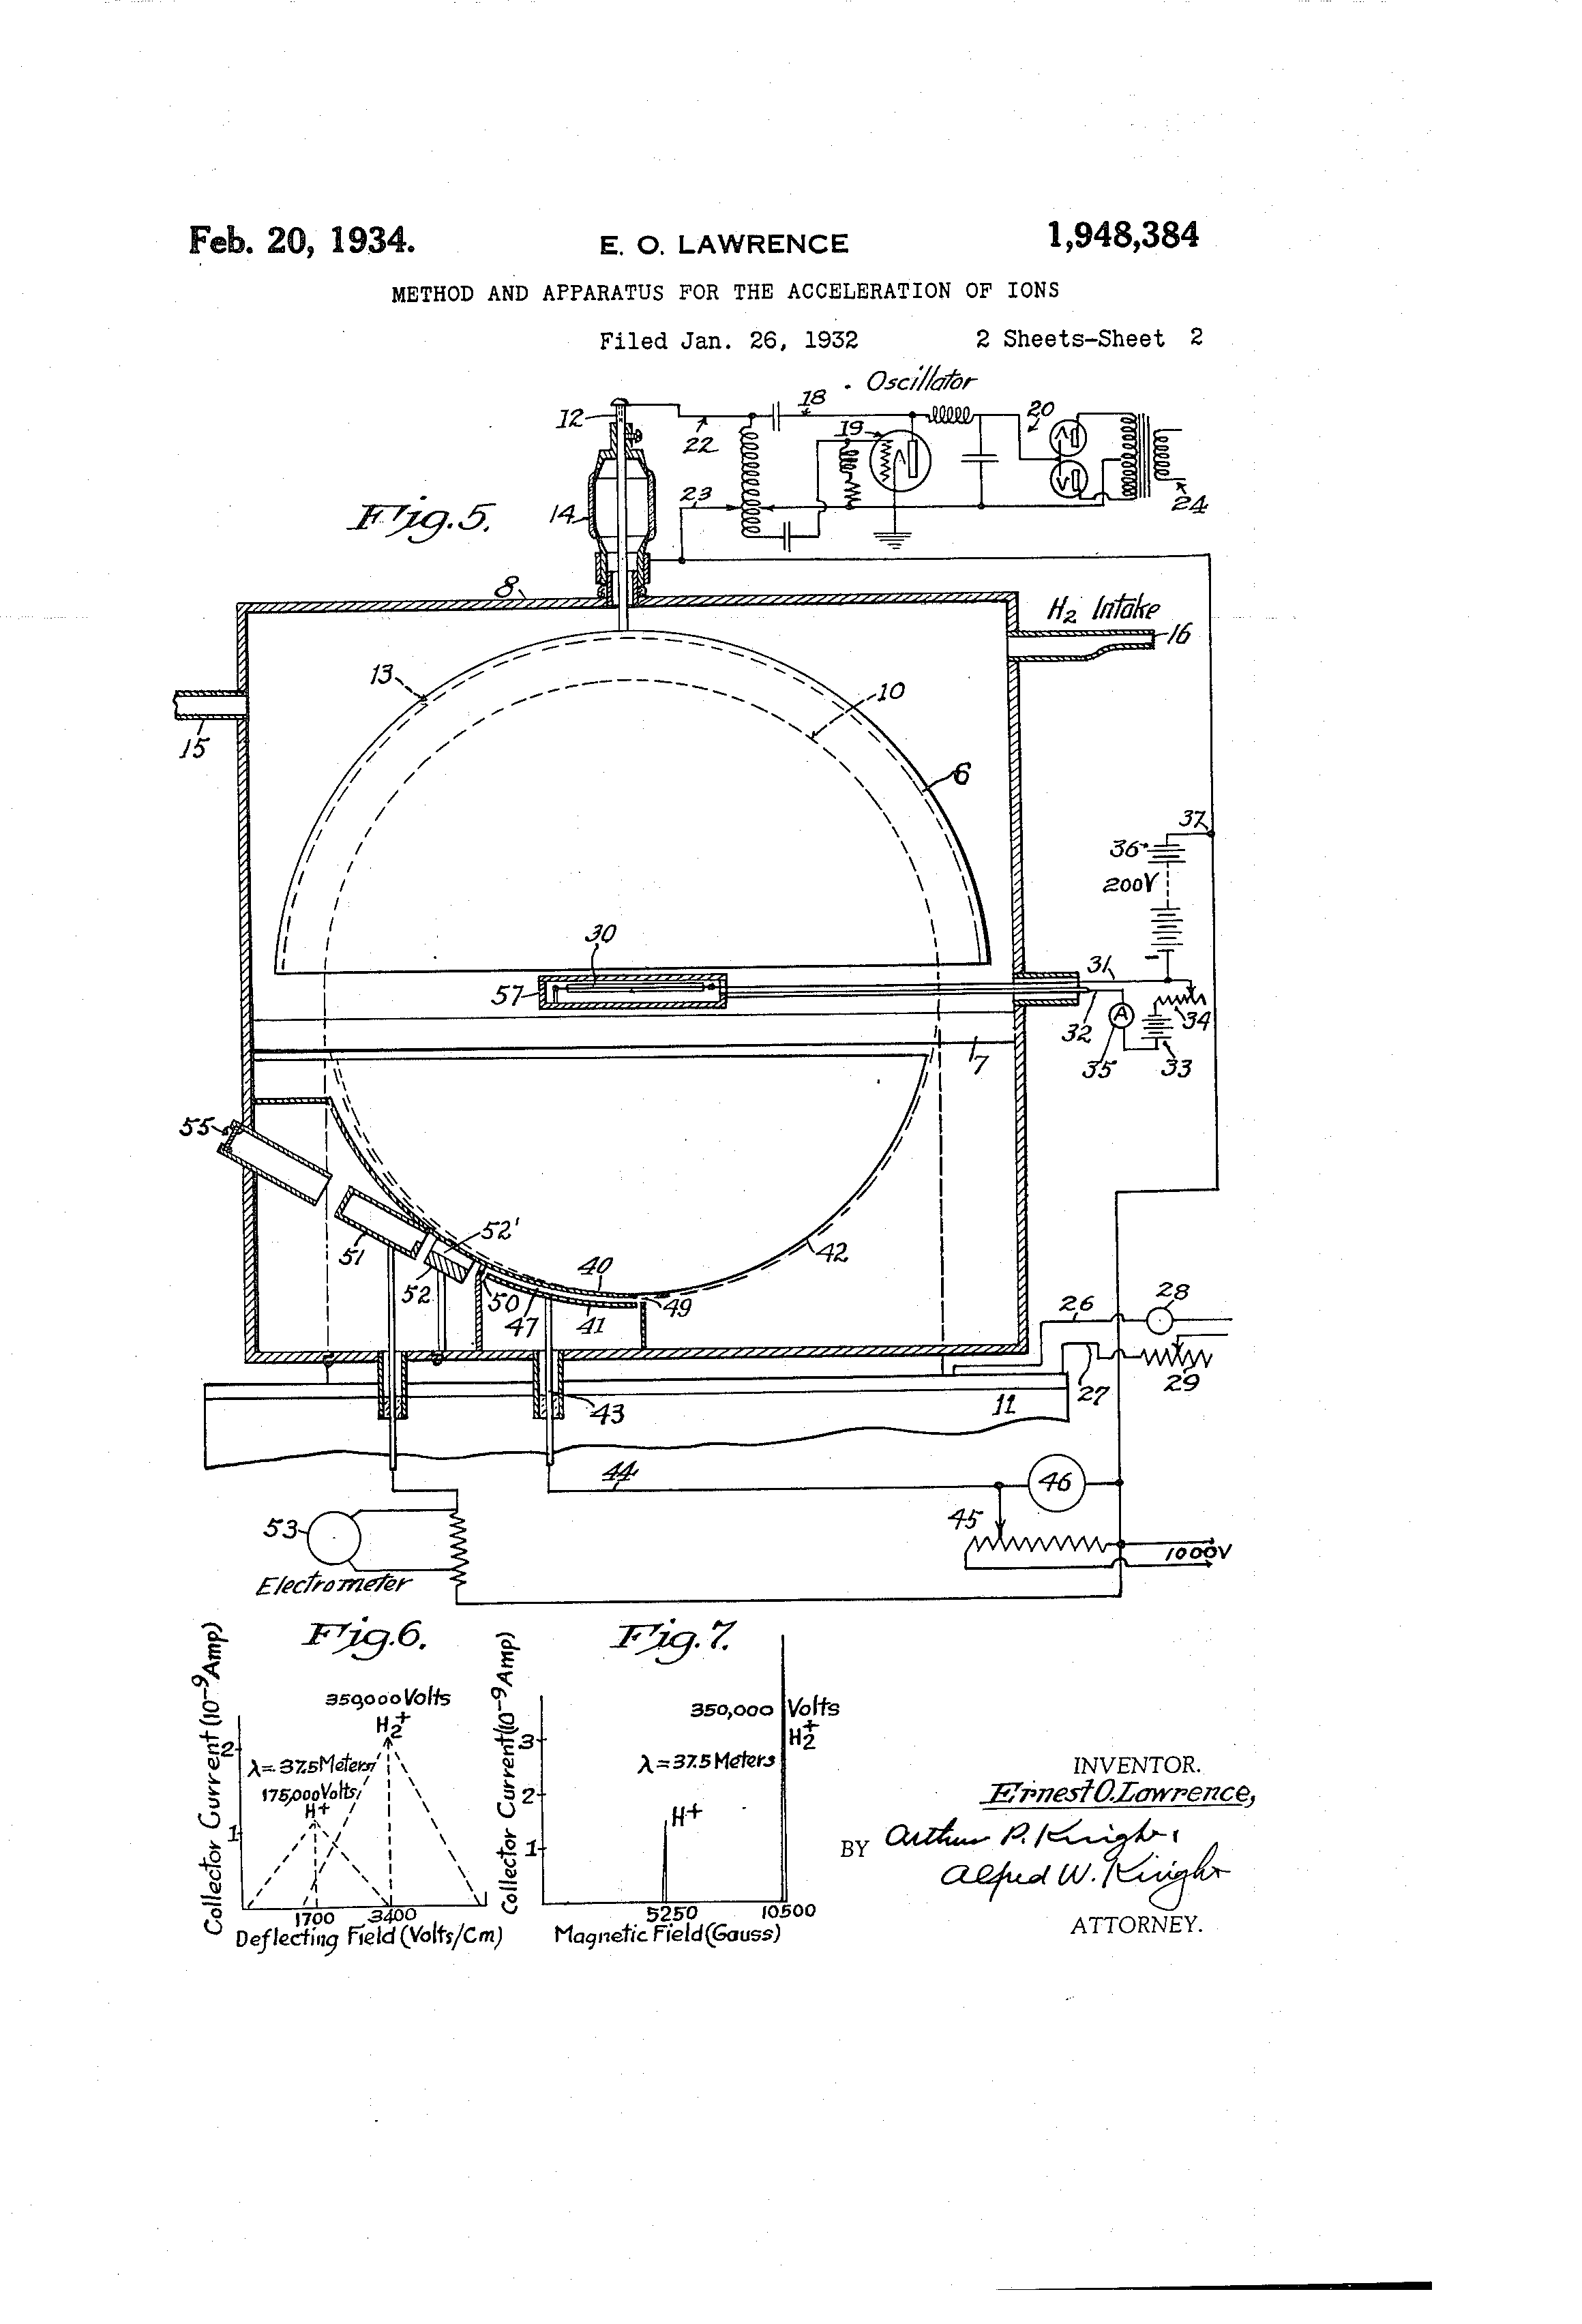
\includegraphics[width=.49\textwidth]{Pictures/cyclo2.png}
  	\caption{\label{fig:cyclo}
                  E. O. Lawrence patent of the cyclotron in the U.S.A.}
  \end{minipage}
\end{figure}

\begin{figure}
 \centering
  \begin{minipage}{\textwidth}
   \centering
    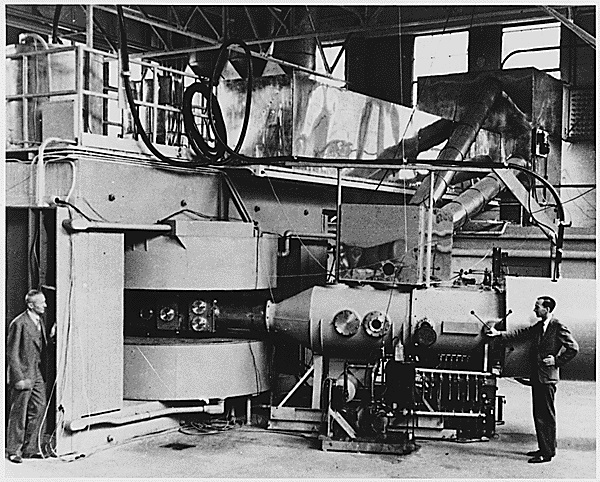
\includegraphics[width=.49\textwidth]{Pictures/cyclo3}
  	\caption{\label{fig:lawrence}
   		E. O. Lawrence next to his 1.5 m in diameter cyclotron
                        at LBNL.
                      \footnotesize{Picture from U.S. Department of Energy}}
  \end{minipage}
\end{figure}

% Betatron
Using yet another of Wider\"oe's ideas, Donald Krest built a machine in 1940
that would keep an almost constant orbit while accelerating the electrons. This
is achieved by increasing the magnetic field over time. Betatrons where widely
used in hospitals as sources of X-rays.
% microtron %nothing relevant to say here
% Synchrotron
In 1944 Vladimir Veksler \cite{veksler} and separately in 1945 Edwin McMillan
\cite{PhysRev.McM} published the principles of phase stability which relates the
synchronicity of the orbiting particles and the electric field of the
time-varying RF. Using this principle Frank Goward and D.E. Barnes built the
first synchrotron by modifying an existing betatron in England
\cite{GOWARD1946}. The second synchrotron accelerator was built by General
Electric Research Laboratory (GERL) and it was here were synchrotron radiation
was first observed. This effect will be further discussed in chapter \ref{c:sr}.


Given the large mass of protons compared to electrons, they become
ultrarelativistic at much higher energies, this posses a difficulty to
synchrotrons: They need to increase the magnetic field as they gain energy. This
technological problem had the effect of proton synchrotrons developing much
latter. Te cosmotron was the first synchrotron to achieve the \SI{}{GeV} regime
\cite{cosmotron}, and the first one to use the beam for external experiments
\cite{cosmotron2}.

After the idea of strong focusing was developed, using focusing-defocusing
quadrupole magnets, it became possible to reach even higher energies. The CERN
Proton Synchrotron started operating in 1959, and it reached energies of 28
GeV.

In 1973 at the Stanford Positron Electron Accelerating Ring (SPEAR), researchers
realized that the SR emitted by the beam was too high to allow it to go to
waste, hence creating the Stanford Synchrotron Radiation Laboratory
(SSRL). Although the goal of SSRL was to take advantage of the
`wasted' energy emitted as SR, eventually SPEAR became solely dedicated to SSRL.




%synchtrotron
% Colliders
\section{Working Principles}

\section{LHC}
\subsection{HL-LHC}
\section{FCC}
\subsection{HE-LHC}
\subsection{FCC-hh}
\subsection{FCC-ee}
\subsection{FCC-he}
